\documentclass[11pt,a4paper]{article}
\usepackage{times,latexsym}
\usepackage{url}
\usepackage[T1]{fontenc}

%% Package options:
%% Short version: "hyperref" and "submission" are the defaults.
%% More verbose version:
%% Most compact command to produce a submission version with hyperref enabled
%%    \usepackage[]{tacl2018v2}
%% Most compact command to produce a "camera-ready" version
%%    \usepackage[acceptedWithA]{tacl2018v2}
%% Most compact command to produce a double-spaced copy-editor's version
%%    \usepackage[acceptedWithA,copyedit]{tacl2018v2}
%
%% If you need to disable hyperref in any of the above settings (see Section
%% "LaTeX files") in the TACL instructions), add ",nohyperref" in the square
%% brackets. (The comma is a delimiter in case there are multiple options specified.)

\usepackage[acceptedWithA]{tacl2018v2}
\usepackage{graphicx}

\title{Aspect-based sentiment analysis}

% Author information does not appear in the pdf unless the "acceptedWithA" option is given
% See tacl2018v2.sty for other ways to format author information
\author{
    Miha Bizjak, Anže Gregorc, Rok Grmek \\
    University of Ljubljana \\
    Faculty for computer and information science \\
    Večna pot 113, SI-1000 Ljubljana \\
    mb9232@student.uni-lj.si, ag9497@student.uni-lj.si, rg6954@student.uni-lj.si
}

\date{}



\begin{document}



\maketitle



\begin{abstract}
When performing sentiment analysis on texts mentioning multiple entities, the sentiment towards each of them in not necessarily the same, and it is important to determine what sentiment applies to each entity separately.
In this paper, we study aspect-based sentiment analysis approaches applied to texts in Slovene.
We implement three models. In the first model we use a sentiment lexicon to determine sentiment of words close to an entity, in the same sentence and in the same document and use those as features for a random forest classifier.
In the second model, we add a neural model for dependency parsing to the pipeline and construct features based on words close in a sentence's dependency tree instead of sequentially.
The third model uses BERT embeddings with a neural classifier to construct embeddings.
We evaluate the approaches on the SentiCoref 1.0 corpus of Slovene texts for aspect-based sentiment analysis.
\end{abstract}



\section{Introduction}

Online news, forums and social media are a place for everyone to read and write articles and posts across various domains.
People can also leave comments and giving their opinion and express their feelings about the topics.
That leads  to a huge amount of text content.
That is probably why natural language analysis is currently a hot topic around the world.
We wanted to extract useful information out of large amount of text data.Since we have no time for reading all the words that are written nowadays, we hope to build a good computer program to do that for us.
In this project we chose to do aspect-based sentiment analysis.
Our task is to get the subjective information from text material that refer to a entity with the use of natural language processing and other methods.
An entity is considered as a person, organization or a location and can be represented multiple times in one document or a sentence and there could be more entities in one document.

For the given task, we decided to test multiple approaches and develop different models for predicting the sentiment for each entity.
We will first define some really simple models as a starting point, and then we will try to derive some more complex models.
All of them will be targeting the Slovene language, and we will evaluate each of the models on the Slovene corpus for aspect-based sentiment analysis - SentiCoref 1.0~\cite{zitnik2019slovene}.



\section{Related work}

The main challenge of entity-based analysis is how to find words that describe the entity and identify if contributes to positive or negative sentiment to a given entity.
A lot of related work tried to predict sentiment of the whole document.
But in many cases, a text can describe the polarity of more entities.
That is why we suggest that sentiment analysis is done on entity level.
Since our task is more specific we focused more on methods that identify entities.

In the paper~\cite{ding2018entity} they developed an entity-based sentiment analysis SentiSW and tested it on issue comments from GitHub.
SentiSW can classify issue comments into \emph{<sentiment, entity>} tuples.
They evaluate the entity recognition by manually annotation and it achieves 75\% accuracy.
The main pipeline of this tool is preprocess (words removal, words replacing, stem), feature vectorize (TF-IDF, Doc2vec), classifier (random forest, bagging and other supervised machine learning methods) and entity recognition (rule-based method).

The use of word embeddings provide powerful methods for semantic understanding without the need of creating large amounts of annotated test data.
The paper~\cite{sweeney2017multi} enhanced the word embeddings approach with the  deployment of a sentiment lexicon-based technique to appoint a total score that indicates the polarity of opinion in relation to a particular entity.
They associate a given entity with the words describing it and extracting the associated sentiment to try to infer if the text is positive or negative in relation to the entity.

As stated in the paper~\cite{song2019attentional}, a lot of the existing approaches are modelling context and target words with RNNs and attention.
This paper addresses the issues with RNNs and proposes an Attentional Encoder Network for modeling the semantic interactions between target and context words.
The paper also addresses the label unreliability issue.
The proposed model with the use of pre-trained BERT embedding achieved state-of-the-art results while still being a relatively lightweight model.

Another successful approach that utilizes the BERT model is described in the paper~\cite{sun2019utilizing}.
In this paper, the authors tried a few methods, where they were generating an auxiliary sentence for each prediction.
They basically converted the aspect-based sentiment analysis problem into a sentence-pair classification task.



\section{Methods}

\subsection{Dataset}

The SentiCoref 1.0 dataset contains 837 documents with annotations of named entities (31,419 entities in total) and sentiment annotations for each entity. For each entity, a sentiment value from 1 to 5 is assigned. The distribution of sentiment labels in the dataset is shown in Table~\ref{tab:sentiment_distribution}.

\begin{table}[h]
\centering
\begin{tabular}{ll}
Sentiment label   & Entity count \\ \hline
1 - Very negative & 30           \\
2 - Negative      & 1801         \\
3 - Neutral       & 10869        \\
4 - Positive      & 1705         \\
5 - Very positive & 24          
\end{tabular}
\caption{Entity sentiment distribution in the SentiCoref 1.0 dataset.}
\label{tab:sentiment_distribution}
\end{table}

\subsection{Models}

All developed models are described in this section.
First two models are really simple and have no practical use - we implemented them as a starting point in order to test the entire evaluation framework, and to have a reference performance for comparing other more complex models.

\subsubsection{Random model}

The Random model simply assigns random sentiment (1 - 5) to each entity, without knowing anything about the actual sentiment.
Assigned sentiments are uniformly distributed, and even the distribution of the sentiments in the dataset was not taken into account.
We are expecting that this model would serve as a reference for the lowest possible evaluation performance.

\subsubsection{Majority model}

The Majority model assigns neutral sentiment (3) to all entities.
The idea for this model came from a fact that around 75\% of the entities in the dataset are labeled with the neutral sentiment.
Therefore, we are expecting decent performance because of the distribution of the sentiments in the dataset.
We will also use this performance as a reference for comparing other models.
More complex models are expected to extract more knowledge from the given data, and they should be performing better than this one.

\subsubsection{Lexicon Features model}

For the first machine learning model we tried to build it using hand-crafted features. 
To do that, we used opinion lexicons with positive and negative words typical for Slovenian language.
We used manually translated opinion lexicon used in~\cite{kaduncanaliza}.
It contains 62,148 negative word forms and 27,681 positive word forms.


Using SentiCoref dataset and lexicon we implemented different hand-crafted features that we thought they can provide some kind of sentiment indicators for each entity.
One sample that is forwarded to machine learning model describes one entity of a particular document with the following features:
\begin{itemize}
    \item number of positive words up to \emph{n\_pos} words before and after (around) current entity occurrence,
    \item number of negative words up to \emph{n\_neg} words around current entity occurrence,
    \item number of positive words for which the current entity is the closest,
    \item number of negative words for which the current entity is the closest,
    \item number of positive words where it is only current entity in a sentence,
    \item number of negative words where it is only current entity in a sentence,
    \item number of positive words in the text,
    \item number of negative words in the text,
    \item number of different entities in the text,
    \item number of occurrences of the entity.
\end{itemize}

Sentence splitting is done using the pretrained Punkt sentence tokenizer~\cite{kiss2006unsupervised} for Slovene provided with the \texttt{nltk} Python package~\cite{bird2009natural}.

We tried different numbers of \emph{n\_pos} and \emph{n\_neg} to represent features. 
For example, we used [3, 5, 10] for \emph{n\_pos} one sample, therefore we generated 3 column features.
We also normalized features in some cases. 
Since the features can have different range of values this can provide better results.
In the results section we described what set of features suited us the most.

For a machine learning model we could use a numerous models such as Nearest Neighbours, \emph{SVM}, Naive Bayes.
We selected Random Forest (\emph{RF}) model since it performs quite well in most cases.
Parameters that we focused for building \emph{RF} are the number of trees in the forest, the function to measure the quality of a split (we tried Gini impurity and information gain) and the maximum depth of a tree. 
The optimal parameters for the model are chosen using grid-search with 5-fold cross-validation.


\subsubsection{Dependency model}

The dependency parsing model attempts to improve on the lexicon features model by using word dependency information within sentences.

For dependency parsing, we use the Stanza library~\cite{qi2020stanza} with the pretrained model for Slovene. The model was trained on the Universal Dependencies Treebank for Slovenian~\cite{dobrovoljc2017universal}.

The Stanza pipeline takes tokenized sentences as input and outputs sentences annotated with lemmas, part-of-speech tags and dependency information.

Each document is split into sentences, then the sentences are analyzed using the Stanza pipeline to obtain the dependency tree.
Using the dependency information, we then calculate distances between each positive/negative word - entity pair.
Similar to the lexicon features model, we then construct a feature vector for each entity. We count for how many positive/negative words a specific entity is the closest in the dependency trees, and how many positive/negative words are within $N$ distance in the tree, one feature for positive words and one feature for negative words within each distance.

We expect dependency tree distances to more accurately determine which positive/negative words correspond to which entities compared to regular distances, especially in cases such as nested sentences.

\subsubsection{BERT model}

The well known BERT (Bidirectional Encoder Representations from Transformers) model~\cite{devlin2018bert} can be used for variety of natural language processing tasks, including the sentiment analysis.
We decided to utilize the pre-trained multilingual BERT embedding layers and combine them with additional convolutional layers and some dense layers at the end for direct classification of the sentiment.

In order to prevent to much variation in the length of inputs (the number of mentions can vary significantly from entity to entity), we presented the idea of treating each mention of an entity as a separate learning case.
Therefore we constructed a training set such that each input was represented with a set of words from the neighbourhood of the entity mention, and each output was a sentiment class (1 - 5) of the mentioned entity.
In the prediction stage, where the goal is to predict the sentiment for the entity and not for all individual mentions of the entity, we decided to sum predictions over all mentions of the entity, and we select the class with maximum support.
The main assumption here was, that all mentions of an entity has similar (hopefully equal) sentiment.
Therefore, we may expect some issues if an entity would have extremely negative sentiment in some mentions and extremely positive sentiment in other mentions, but the average sentiment for this entity would be labeled neutral in our dataset.
In this case, we would also assign neutral sentiment to all mentions of this entity when constructing the training samples, although some sentiments could be extremely negative or extremely positive.

The architecture of our model is shown in Figure~\ref{fig:bert-model}.
The model is roughly constructed from three parts - first part converts a sequence of words into word embeddings, where the pretrained BERT is used; the second part is convolving with different filters over the sequence of embeddings; and the third part is used for classifying the features, that were extracted with the convolution, into one of the five sentiment classes.

\begin{figure}[h!]
\centering
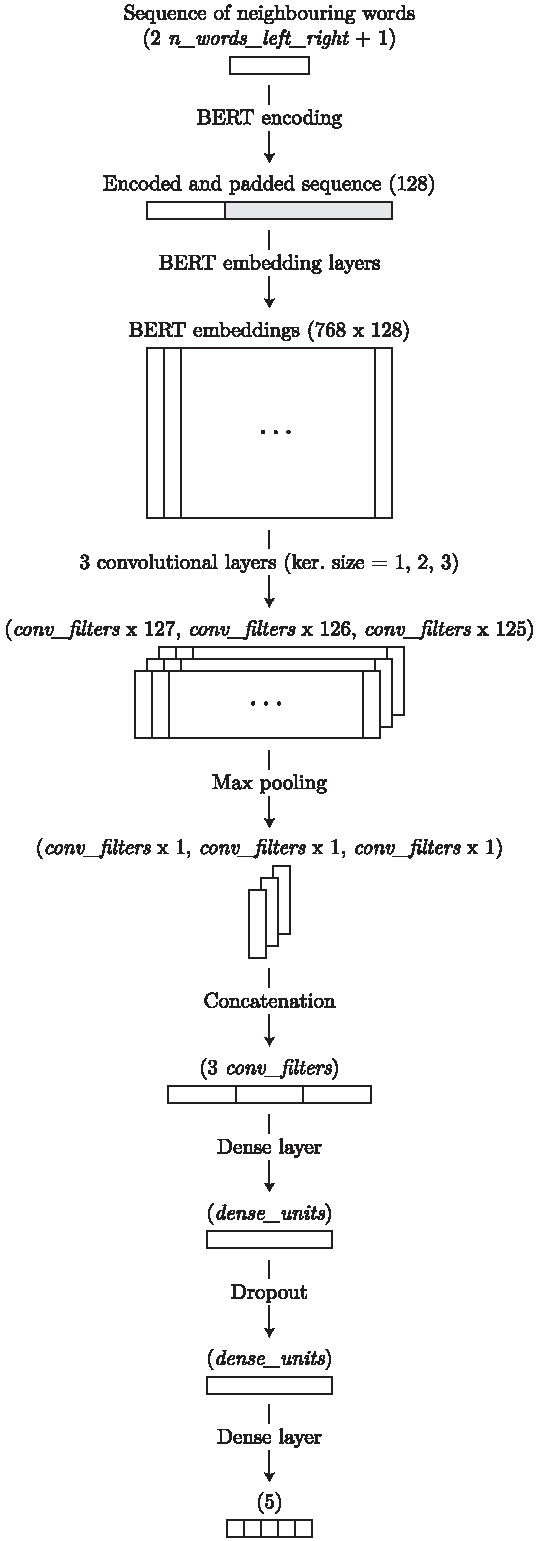
\includegraphics[width=1.0\columnwidth]{bert-model.pdf}
\caption{Architecture of the BERT model.}
\label{fig:bert-model}
\end{figure}

The sequence of words is first extracted from the neighbourhood of the entity mention (parameter \textit{n\_words\_left\_right} defines how many words to the left and right are used).
Then before using the BERT embedding layers, we encode the sequence of words and pad the sequence to a fixed length of 128.
After obtaining the BERT embeddings, we use three parallel convolutional layers with \textit{conv\_filters} number of filters, where the kernels are of sizes 1, 2 and 3 correspondingly.
To each filter we apply the max pooling, and then we concatenate the results into a vector of size $3 \cdot \textit{conv\_filters}$.
The concatenated vector is then put through the dense layer with \textit{dense\_units} number of neurons, then we apply the dropout to prevent overfitting, and lastly we use the dense layer with 5 neurons and the softmax activation for the final classification (other neurons are using the relu activation).

The model fitting procedure was done with different dropout rates (parameter \textit{dropout\_rate}) in batches of size \textit{batch\_size}, and with \textit{epochs} number of training repetitions.
During the fitting, the weights from BERT embedding layers were not updated.

\subsection{Evaluation}

Evaluation was performed on the SentiCoref 1.0 dataset, using a randomized 0.67/0.33 train/test split on the documents.
For each model, we measured the F1 score, precision, recall and RMSE metrics.
The metrics were calculated using the \texttt{sklearn} library with the \texttt{average="weighted"} parameter, i.e. calculated for each label and then averaged, weighted by the number of true instances for each label.
% \begin{itemize}
%     \item 2/3 train, 1/3 test split
%     \item Implemented measures: Accuracy, Precision, Recall, F1 score.
% \end{itemize}



\section{Results}

In this section we are presenting the results of evaluation of all tested models.
In Table~\ref{tab:rnd-maj-results}, the results of first two simple models are given as a reference for comparing the results of other models, described in the following subsections.

\begin{table}[h]
\centering
\begin{tabular}{ccccc}
    & F1 score & Precision & Recall & RMSE   \\ \hline
Rnd & 0.2764   & 0.5976    & 0.2011 & 1.4912 \\
Maj & 0.6461   & 0.5661    & 0.7524 & 0.5058
\end{tabular}
\caption{Evaluation results of the Random model and the Majority model.}
\label{tab:rnd-maj-results}
\end{table}

\subsection{Lexicon Features model}

The results of the Lexicon Features model are shown in Table~\ref{tab:lexicon-features-results} and~\ref{tab:lexicon-features-parameters}.
We can see that results do not vary a lot. 
If we look closely enough we see that models without normalization performed slightly worse.
We could say that the best model is the model with \emph{key} 2. 
That is not quite surprising since it contains 6 features that indicate positive and negative sentiments around entity and here we also normalize features.
All the other models have less number of features (\emph{n\_pos} and \emph{n\_neg}). 

Compared to Random and Majority model we can conclude that our hand-crafted features provide some information about entity sentiment.
Lexicon Features model performed better on all the metrics compared to Random model.
The Majority model performed slightly better when we talk about Recall and RMSE most probably because we have very imbalanced dataset.
Despite the fact that the dataset is imbalanced, all the variations of Lexicon Features have better F1 score and Precision so we would still rather use Lexicon Features model in real world.


\begin{table}[h]
\centering
\begin{tabular}{ccccccc}
\emph{key} & F1 score & Precision & Recall & RMSE   \\ \hline
1 & 0.6742   & 0.6676    & 0.7477 & 0.5312 \\
2 & 0.6768   & 0.6827    & 0.7522 & 0.5225 \\
3 & 0.6764   & 0.6730    & 0.7498 & 0.5272 \\
4 & 0.6768   & 0.6719    & 0.7479 & 0.5261 \\
5 & 0.6730   & 0.6673    & 0.7467 & 0.5296 \\
6 & 0.6689   & 0.6608    & 0.7447 & 0.5298 \\
\end{tabular}
\caption{Evaluation results of the Lexicon Features model. Because the table would be too wide we split the table in two parts. The other part is in Table~\ref{tab:lexicon-features-parameters} and describes parameters for this results. }
\label{tab:lexicon-features-results}
\end{table}

\begin{table}[h]
\centering
\begin{tabular}{cccc}
\emph{key} & \emph{n\_pos} & \emph{n\_neg} & Norm \\ \hline
1 & (5) & (5) & F  \\
2 & (3,5,10) & (3,5,10) & T \\
3 & (3,5,10) & (3,5,10) & F  \\
4 & (3,5,10) & (3) & T  \\
5 & (5) & (3,5,10) & T  \\
6 & (3,15) & (10,15) & F \\
\end{tabular}
\caption{Parameters for each model shown in Table~\ref{tab:lexicon-features-results}.
        The parameter norm represents weather we normalized features before we put to the model (T) or not (F). The parameters \emph{n\_pos} and \emph{n\_neg} are described in Models section. In summary, if we have 3 numbers in \emph{n\_pos} column, that means we used 3 features (columns in data set) that count positive words around entity. }
\label{tab:lexicon-features-parameters}
\end{table}

\subsection{Dependency model}

The results for the dependency model are shown in Table~\ref{tab:dependency-results}.

% \begin{table}[h]
% \centering
% \begin{tabular}{cccc}
% F1 score & Precision & Recall & RMSE   \\ \hline
% 0.6778   & 0.6711    & 0.7458 & 0.5273 \\
% \end{tabular}
% \caption{Evaluation results of the dependency model.}
% \label{tab:dependency-results}
% \end{table}

\begin{table}[h]
\centering
\begin{tabular}{ccccccc}
\emph{key} & F1 score & Precision & Recall & RMSE   \\ \hline
1 & 0.6733   & 0.6612    & 0.7396 & 0.5359 \\ %3t
2 & 0.6765   & 0.6676    & 0.7441 & 0.5328 \\ %3f
3 & 0.6767   & 0.6653    & 0.7435 & 0.5369 \\ %123t
4 & 0.6739   & 0.6679    & 0.7439 & 0.5277 \\ %123f
5 & 0.6767   & 0.6721    & 0.7476 & 0.5302 \\ %12345t
6 & 0.6811   & 0.6784    & 0.7493 & 0.5245 \\ %12345f
\end{tabular}
\caption{Evaluation results of the dependency model. The parameters used for each model are shown in Table~\ref{tab:dependency-parameters}}
\label{tab:dependency-results}
\end{table}

\begin{table}[h]
\centering
\begin{tabular}{ccc}
\emph{key} & \emph{N} & Norm \\ \hline
1 & (3) & T  \\
2 & (3) & F  \\
3 & (1,2,3) & T  \\
4 & (1,2,3) & F  \\
5 & (1,2,3,4,5) & T  \\
6 & (1,2,3,4,5) & F  \\
\end{tabular}
\caption{Parameters for each model shown in Table~\ref{tab:dependency-results}.
        The parameter norm represents weather we normalized features before we put to the model (T) or not (F). The parameter \emph{N} represents the list of distances used to calculate sentiment close in the dependency tree. }
\label{tab:dependency-parameters}
\end{table}

The model performs similarly to the Lexicon Features model. With the best set of parameters (model 6) we achieve only slightly better values compared to the Lexicon Features model, which shows that in certain cases using the dependency tree neighborhood helps assign the sentiment to the correct entity.
Despite that, we still fail to achieve better values than the Majority model for Recall and RMSE, and calculating the dependencies for each sentence requires additional computation.

\subsection{BERT model}

The model was developed with variety of free parameters.
We tested different configurations in order to see the impact of each parameter on the model performance.
For the starting point we set the parameters as follows: \textit{n\_words\_left\_right}: 6, \textit{conv\_filters}: 100, \textit{dense\_units}: 256, \textit{dropout\_rate}: 0.2, \textit{batch\_size}: 128, \textit{epochs}: 5.
Then we evaluated several experiments were we were changing one parameter at a time and left all others fixed.
All the results are given in Tables~\ref{tab:bert-results-1},~\ref{tab:bert-results-2},~\ref{tab:bert-results-3},~\ref{tab:bert-results-4},~\ref{tab:bert-results-5},~\ref{tab:bert-results-6} and in Figure~\ref{fig:bert-model-results}.

\begin{table}[h]
\centering
\begin{tabular}{ccccc}
  & F1 score & Precision & Recall & RMSE   \\ \hline
1 & 0.6459   & 0.5844    & 0.7503 & 0.5072 \\
2 & 0.6541   & 0.6131    & 0.7495 & 0.5124 \\
3 & 0.6470   & 0.6103    & 0.7474 & 0.5126 \\
4 & 0.6628   & 0.6348    & 0.7250 & 0.5544 \\
5 & 0.6631   & 0.6383    & 0.7233 & 0.5597 \\
6 & 0.6734   & 0.6519    & 0.7114 & 0.5812 \\
7 & 0.6692   & 0.6465    & 0.7083 & 0.5775
\end{tabular}
\caption{Evaluation results of the BERT model with respect to parameter \textit{n\_words\_left\_right}.}
\label{tab:bert-results-1}
\end{table}

\begin{table}[h]
\centering
\begin{tabular}{ccccc}
    & F1 score & Precision & Recall & RMSE   \\ \hline
50  & 0.6596   & 0.6455    & 0.7330 & 0.5527 \\
100 & 0.6734   & 0.6519    & 0.7114 & 0.5812 \\
150 & 0.6625   & 0.6364    & 0.7068 & 0.5835
\end{tabular}
\caption{Evaluation results of the BERT model with respect to parameter \textit{conv\_filters}.}
\label{tab:bert-results-2}
\end{table}

\begin{table}[h]
\centering
\begin{tabular}{ccccc}
    & F1 score & Precision & Recall & RMSE   \\ \hline
64  & 0.6461   & 0.5661    & 0.7524 & 0.5058 \\
128 & 0.6585   & 0.6305    & 0.7262 & 0.5527 \\
256 & 0.6734   & 0.6519    & 0.7114 & 0.5812
\end{tabular}
\caption{Evaluation results of the BERT model with respect to parameter \textit{dense\_units}.}
\label{tab:bert-results-3}
\end{table}

\begin{table}[h]
\centering
\begin{tabular}{ccccc}
    & F1 score & Precision & Recall & RMSE   \\ \hline
0.1 & 0.6745   & 0.6510    & 0.7131 & 0.5815 \\
0.2 & 0.6734   & 0.6519    & 0.7114 & 0.5812 \\
0.3 & 0.6686   & 0.6525    & 0.6905 & 0.6077
\end{tabular}
\caption{Evaluation results of the BERT model with respect to parameter \textit{dropout\_rate}.}
\label{tab:bert-results-4}
\end{table}

\begin{table}[h]
\centering
\begin{tabular}{ccccc}
    & F1 score & Precision & Recall & RMSE   \\ \hline
32  & 0.6533   & 0.6237    & 0.7410 & 0.5260 \\
64  & 0.6592   & 0.6380    & 0.7334 & 0.5440 \\
128 & 0.6734   & 0.6519    & 0.7114 & 0.5812
\end{tabular}
\caption{Evaluation results of the BERT model with respect to parameter \textit{batch\_size}.}
\label{tab:bert-results-5}
\end{table}

\begin{table}[h]
\centering
\begin{tabular}{ccccc}
   & F1 score & Precision & Recall & RMSE   \\ \hline
5  & 0.6734   & 0.6519    & 0.7114 & 0.5812 \\
10 & 0.6750   & 0.6570    & 0.7015 & 0.6005 \\
15 & 0.6636   & 0.6548    & 0.6743 & 0.6430
\end{tabular}
\caption{Evaluation results of the BERT model with respect to parameter \textit{epochs}.}
\label{tab:bert-results-6}
\end{table}

\begin{figure}[h!]
\centering
\includegraphics[width=1.0\columnwidth]{bert-model-results.png}
\caption{Evaluation results of the BERT model.}
\label{fig:bert-model-results}
\end{figure}

Similar trade-off between precision and recall is seen in all experiments.
Parameter configurations, evaluated with higher recall (bot lower precision) are performing similarly as the Majority model - most predictions are targeting the neutral sentiment and very few predictions are made for the other four sentiment classes.
The other extreme with higher precision (but lower  recall) more likely predicts the non-neutral classes, and in most cases this also results in an overall higher F1 score.
In this kind of trade-off situation we may want to simply trust the F1 score for determining the best performing parameter configuration, as it takes both precision and recall into account, but we noticed an interesting correlation between the F1 score and the RMSE.
Higher F1 score in most cases also resulted in a higher RMSE, which means more error according to the distance between the predicted and the actual class.
This means that one extreme (both F1 score and RMSE high) will more likely predict the edge sentiment classes, but in this case we will more likely fail in some situations when we are dealing with the neutral sentiment.
Another extreme (both F1 score and RMSE low) will offer a more stable model with more predictions quite close to an actual class, but this model won't be so informative as it may never predict the edge sentiment classes.



\section{Discussion}

In this paper we studied the problem of selecting sentiment for different entities in documents provided from dataset SentiCoref  1.0.
We found several challenges to this problem and proposed different solutions to address them. 
In particular, we implemented 3 different approaches of classifying the aspect-based sentiments, one with hand-crafted features, the model with word dependency information and the model built upon the state-of-the-art BERT model. 
All the models resulted to quite similar values (F1 score varies from around 0.64 to 0.68) so we can not select one best model. 
Our conclusion is that we can use a model based on our preferences. 
If we wanted to pick model based on F1 score we could use Dependency model but if we wanted less error according to the sentiment distance we would check on RMSE measure and pick BERT model. 

Because of the distribution of the data, we observe that our models tend to learn to overpredict the neutral sentiment class, which minimizes the amount of significant mistakes, however it also means that the accuracy does not significantly improve compared to the majority model.

In further experiments, we could attempt to combine the hand-crafted features and the BERT embeddings. 
In the hand-crafted features we could add more different features that hopefully contain additional information of sentiment for a particular entity. 
Additionally, undersampling could be performed on the neutral class to improve the training of the models.
We could also expand our dataset with different languages and analyse how models behave in multi-language dataset.




\section{References}

\bibliography{bibliography}
\bibliographystyle{acl_natbib}



\end{document}
